\chapter{Introduction}
\label{sec:intro}

The industrial background of this thesis and its practical implications.
Border 6 and NSI.

\section{Intradomain Routing and TE}
A brief intro to intra-domain routing, BGP, alternatives to BGP such as LISP, overlay networking.
Scope our research under BGP as the routing protocol.

Biblio on the past researches and common practices on interdomain TE with BGP.
Traffic steering method: local pref and prefix split for outbound traffic steering; inbound tricks such as AS-path, community are not certain, and less fine grained. Focus on outbound TE.
System design and route selection methods: common practice (related to policies) and research proposals mainly Akella~\cite{Akella2008}.

Introduce the notion of measurement-based intradomain TE and declare it as the topic and context of this thesis.

\section{Motivations for measurement-based intradomain TE}
To help improve a working system/product for interdomain TE.
What remains to be done or what's the gap between these research proposals and a working system.

\section{Building blocks of measurement-based TE}
The building blocks of the systems and remaining challenges.

\begin{figure}[!htb]
\centering
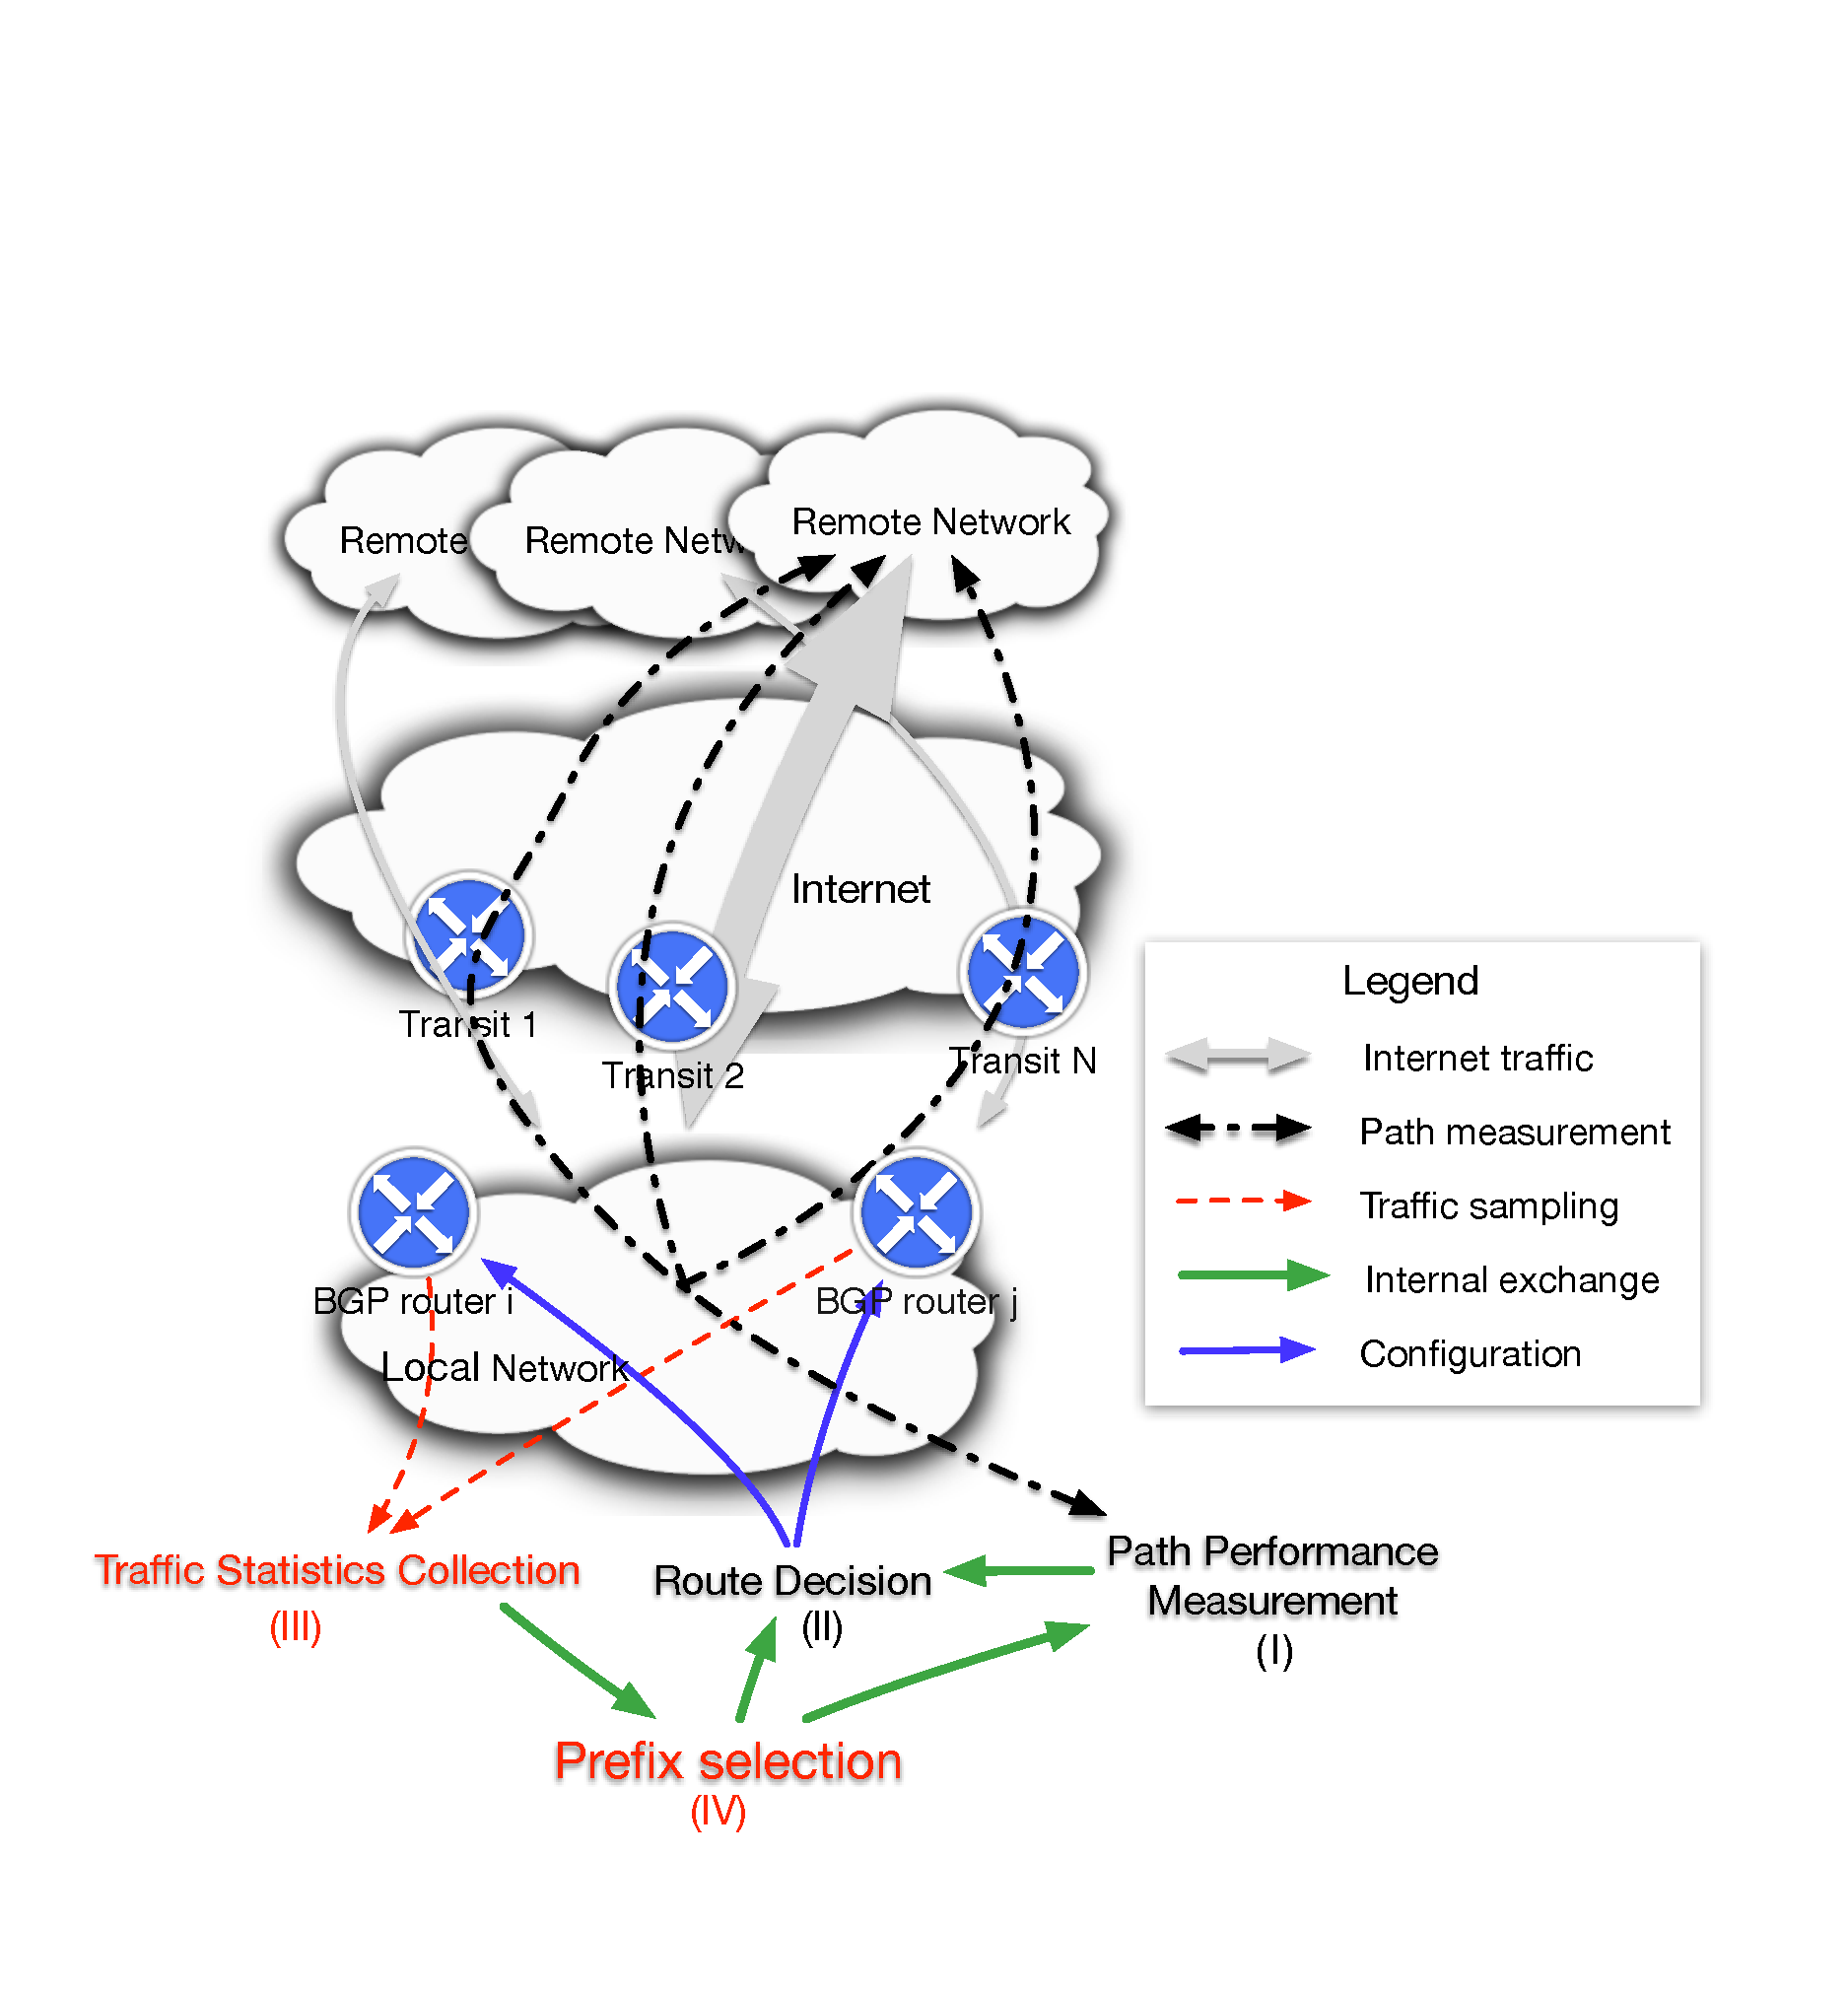
\includegraphics[width=0.9\textwidth]{gfx/chap1/archi.pdf}
\caption{Building blocks of measurement-based inter-domain TE system.}
\label{fig:archi}
\end{figure}

\section{Prefix selection: focus on most important destinations}
Measurements on traffic volumes.
Why we need to focus on most import destinations (a scalability issue), how we did it (NOMS).

\section{RTT measurements with RIPE Atlas}
Measurements on Round-Trip time.
\subsection{RIPE Atlas}
For the sake of reproducibility, use RIPE Atlas as measurement sources.
Intro to RIPE Atlas.
Measurement quality concerning RIPE Atlas.
\subsection{Measurement quality}
Quality issue from the platform (CoNext).
Measurement differences among multiple probes toward a same destination prefix.(AnNet)
Implication to interdomain TE and what we propose.
\subsection{Synchronized RTT change}
Synchronized RTT changes. Time-series clustering.
Motivation for change detection.

\section{Change detection for RTT measurements}
Detect RTT changes (ITC).
Motivation for RTT change detection.

\section{Inferring the location of RTT changes}
The case where probes can not be identified in destination prefixes.
Infer the occurrence of intermediate RTT changes and their locations.
Implication and usage beyond TE.  
